\chapter{Power Analysis}
\graphicspath{{foto/Chap3/}}

The following analysis is based on the assumption that only one operation at time is carried out. The power consumption in the case of contemporary operations, being the register file a multi-port device, will be equal to the sum of the single contributions.
 
\section{Capacitance modeling}
The considered capacitances are the following:
\begin{itemize}
	\item $C_{g,access}$ gate capacitance of a generic pass transistor
	\item $C_{d,access}$ "drain/source" capacitance of a generic pass transistor
	\item $C_{g,rowpass}$, $C_{g,blockpass}$ gate capacitance of internal and external block pass transistors
	\item $C_{d,rowpass}$, $C_{d,blockpass}$ drain capacitance of internal and external block pass transistors
	\item $C_{wl,wire}$ wire capacitance per unit length of wordline
	\item $C_{bl,wire}$ wire capacitance per unit length of bitline
	\item $C_{block,dec},C_{row,dec}$ total capacitances of each type of decoder
	\item $C_{SA,in}$ input capacitance of the sense amplifier
	\item $C_{g,pre}$, $C_{s,pre}$ gate and source capacitance of the precharge transtistor
	\item $C_{ext,pu\_driver}$ external precharge unit driver capacitance
	\item $C_{g,equalizer}$ gate capacitance of the equalizer mos
\end{itemize}

Other useful parameters are:

\begin{itemize}
	\item $N_{bit}$ number of bit for each row, equal to the number of column; 
	\item $N_{wl}$ number of wordlines
	\item $BL_{length}$ length of bitline 
	\item $WL_{length}$ length of wordline
	\item $N_{block}$ number of block
	\item $N_{erase}$ number of erase cycles
\end{itemize}

\subsection{Precharge block capacitances}

To evaluate power dissipation of the precharge block, the following capacitance is considered: 

\[
C_{prec}=C_{ext,pu\_driver}+2 \cdot C_{g,pre}+C_{g,equalizer}
\]

\subsection{Lines capacitances}
\label{subsec:capacitance}

To accurately evaluate the capacitance of the lines ($C_{bl}$ and $C_{wl}$), the capacitance of the wires and the length of bitline/wordline are considered. So the total capacitance for each line is:

\[
C_{wl} = C_{d,rowpass} + 2 \cdot C_{g,access} \cdot N_{bit} + WL_c \cdot WL_{length}
\]

\[
C_{bl}= C_{s,pre} + C_{d,access} \cdot N_{wl} + BL_c \cdot BL_{length} +C_{SA,in}
\]

\[
C_{bl,write}= C_{d,driver} + C_{d,access} \cdot N_{wl} + BL_c \cdot BL_{length}
\]

The capacitance $C_{bl,write}$ is similar to the $C_{bl}$, but without the contribution of the precharge block and the sense amplifier capacitances and with a driver load.\\

where $C_{SA,in}$ is the input capacitance of the sense amplifier
\subsection{Decoders capacitance}
\label{subsec:dec_capacitance}
To evaluate the capacitance of the decoders, the following formulas are used:
\[
C_{block,dec}=C_{d,bdec,pcharge}+C_{d,bdec,eval}+C_{g,bdec,inv_{p}}+C_{g,bdec,inv_{n}}
\]

\[
C_{block,stack}=0.5 \cdot C_{g,bdec,n} \cdot Block\_Address \cdot N_{block};
\]

where $C_{g,dec,eval}, C_{d,bdec,pcharge}$ and $C_{d,bdec,eval}$ are, respectively, the gate/drain capacitance of the precharge and evaluation transistors, while the others are the gate capacitances of the output inverter.
In particular, $C_{d,bdec,eval} = Block\_Address \cdot C_{d,bdec,n}$.\\
$C_{block,stack}$ is the equivalent gate capacitance, that has to be loaded to turn on the n-mos and select the correct output, given certain selection bits from the address.\\
Similar expressions have been used for row decoder.
\subsection{Sense Amplifier}
\label{subsec:dec_capacitance}
To evaluate the capacitance of the sense amplifier, the following formulas are used:
\[
C_{SA,in}=C_{d,sa,p}+C_{d,sa,n}+C_{g,sa,p}+C_{g,sa,n}
\]

\section{Read power}
\label{sec:read_power}

\subsection{Decoding stage}
\label{sec:decoding_stage}
During a read operation, the block decoder selects the block in which the operation has to be carried out.
At the same time the row decoder is working to select the addressed word.
The formulas to calculate energy consumption in the decoding phase are the following:
\[
E_{block,dec}= 0.5 \cdot C_{block,dec} \cdot V_{on,pt}^2
\]
\[
E_{stack,bdec}=0.5 \cdot C_{block,stack} \cdot V_{on,pt}^2
\]

\[
E_{row,dec}= 0.5 \cdot C_{row,dec} \cdot (V_{sel}^2+ V_{unsel}^2 \cdot (N_{wl}-1)) \cdot N_{block}
\]
\[
E_{stack,rdec}=0.5 \cdot C_{row,stack} \cdot V_{on,pt}^2 \cdot N_{block}
\]

The energy consumption linked to the selection of the correct block:
\[
E_{row,pt}= 0.5 \cdot (C_{g,rowpass} \cdot N_{wl} + C_{g,blockpass} \cdot N_{bit}) \cdot V_{on,pt}^2
\]

\subsection{Precharge}
\label{sec:precharge}
To speed up the following operations, in order to reduce the latency, the two bitlines are biased to a specific value $V_{bl,prec}$, by the precharge block. Being $V_{bl,prec}$ the final voltage after the equalization between the BL and the complementary one, the starting voltage of the precharge is two times $V_{bl,prec}$. The other lines are supposed to be biased to ground.\\
The formulas to calculate dissipated energy in the precharge phase are the following:

\[
E_{pre}= 0.5 \cdot C_{prec} \cdot (V_{on,pt}^2) \cdot N_bl
\]

\[
E_{bl}= 0.5 \cdot C_{bl} \cdot V_{bl,prec}^2 \cdot N_{bit}
\]

\subsection{Read operation}
\label{sec:read_op}

The wordline of the selected word is biased to $V_{on,pt}$, in order to make the memory cell accessible, while the voltage on the unselected words is set to ground. It is assumed that the initial voltage of the wordline is 0.\\

The energy to switch the selected and the unselected wordlines is the following:
\[
E_{sel}= 0.5 \cdot C_{wl} \cdot (V_{sel}^2+ V_{unsel}^2 \cdot (N_{wl}-1))
\]

where $V_{on,pt}$ is the voltage to enable the memory cell pass transistors.

The bitlines are at the precharge voltage $V_{bl,prec}$ and can have two different kinds of voltage drop, $V_{rd,1}$ and $V_{rd,0}$. 
Being the two bitlines identical, the energy to read is:
\[
E_{read}=0.5 \cdot C_{bl} \cdot ((V_{bl,prec}-V_{rd,0})^2 + (V_{bl,prec}-V_{rd,1})^2) \cdot N_{bit}
\]

where $V_{bl,prec}-V_{rd,0}$ and $V_{bl,prec}-V_{rd,1}$ are the voltage drops to read '0' and '1'.

\subsection{Sense Amplifier}
\label{sec:sense_amp}

The state change in the bitline is detected using a sense amplifier connected to each line.
The energy consumption related to this stage is given by:

\[
E_{SA}= 0.5 \cdot C_{d,blockpass} \cdot V_{bl,prec} \cdot ((V_{bl,prec}-V_{rd,0}) + (V_{bl,prec}-V_{rd,1})) \cdot N_{bit}
\]

\subsection{Total Dynamic Read Power}
\label{sec:total_power}

Total read energy is computed as summation of all the previous terms.
Assuming $f_{read}$ as read frequency and $E_{read}$as total read energy, total read power can be computed as follows:
\[
P_{read}=E_{read}\cdot f_{read}
\]

\section{Write Dynamic Power}
\label{sec:write_power}

Similar analysis can be done for the write operation. Having the same decoding stage to select the addressed location, same relations can be used: a little difference is present in the $E_{row,pt}$. During the write operation, there is no output transistor selected by the write decoder, as Figure \ref{block_scheme} shows.
\[
E_{row,pt}= 0.5 \cdot (C_{g,rowpass} \cdot N_{wl}) \cdot V_{on,pt}^2
\]

To write a certain word is necessary to load through an external driver the $N_{bit}$ bit and charge the respective bitlines to that value. As previously discussed, this step follows the precharge: the driver forces the correct values on the precharged bitlines, discharging one of the two.\\
Basically, one bitline is charged to a certain voltage and the other one is charged to its complementary voltage. Defining $V_{prog}$ and $V_{unprog}$ respectively as voltage to write a '1' and its complement, the used relation is the following:
\[
E_{prog}=0.5 \cdot C_{bl,write} \cdot (V_{prog}^2+V_{unprog}^2) \cdot N_{bit}
\]

Total write energy is so computed as summation of all the previous terms.
Assuming $f_{read}$ as read frequency and $E_{read}$as total write energy, total write power can be computed as follows:
\[
P_{write}=E_{write}\cdot f_{write}
\]

\section{Simulation results}
As for the delay, to verify the plausibility of our computations we assigned a reasonable value to each of the parameters involved in the equations.\\
The obtained results are reported in the figures below.

\begin{minipage}{\linewidth}
	\centering
	\begin{minipage}{0.4\linewidth}
	\begin{figure}[H]
		\begin{center}
			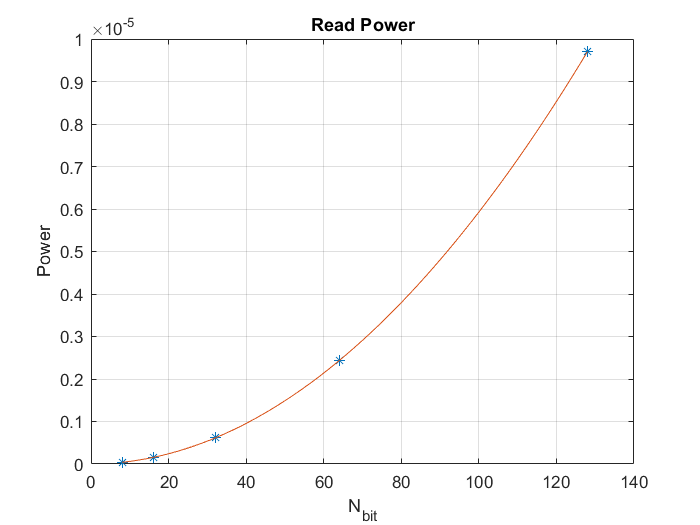
\includegraphics[scale=0.4]{read_test}
		\end{center}
		\caption{Dynamic Power Consumption on a read operation} 
		\label{read_power}
	\end{figure}
	\end{minipage}
	\hspace{0.05\linewidth}
	\begin{minipage}{0.45\linewidth}
	\begin{figure}[H]
		\begin{center}
			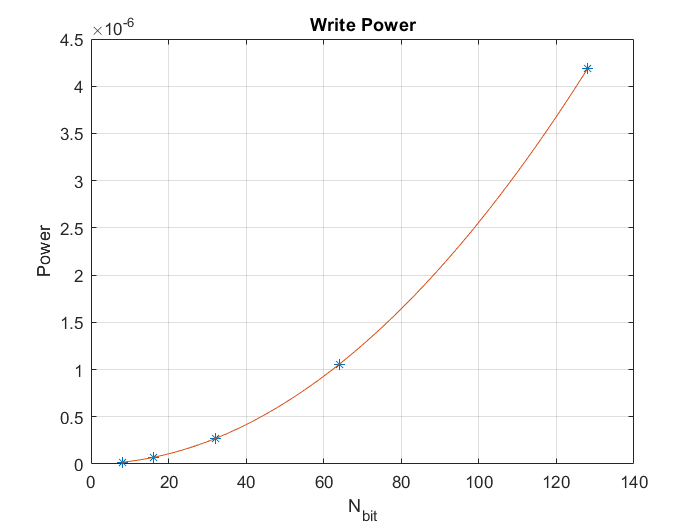
\includegraphics[scale=0.4]{write_test}
		\end{center}
		\caption{Dynamic Power Consumption on a write operation}
		\label{write_power}
	\end{figure}
	\end{minipage}
\end{minipage}
\vspace{0.5cm}

The behaviour represented is reasonable: in all the contributions previously discussed there is a more than linear dependence on $N_{bit}$. In particular the most relevant contributions are dependent from the product of $N_{bit}$ and $BL_{length}$ or $WL_{length}$, that depend linearly by the first one, giving as result a quadratic curve.\\
The curves above show that power consumption for read and write operations is in the order of some $\mu W$, with a slightly larger value for the read  operation, due to the power consumption of the sensing step.\\